\begin{figure}
    \centering
    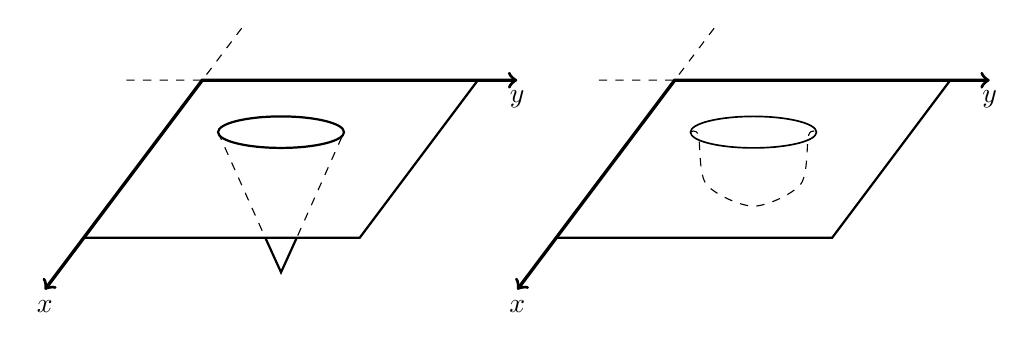
\begin{tikzpicture}
    [scale = 2,
    axis/.style = {<->, very thick},
    dashed line/.style={dashed, thick}]
    \draw[axis](3, 0)node[below]{$y$} -- (1, 0) -- (0, -1.33)node[below]{$x$};
    \draw[dashed](1.25, 0.33) -- (1, 0) -- (0.5, 0);
    \draw[thick](.25, -1) -- (2, -1) -- (2.75, 0);
    \draw[thick] (1.5, -0.33) ellipse (.4 and 0.1);
    \draw[dashed] (1.1, -0.33) -- (1.4, -1) -- (1.6, -1) -- (1.9, -0.33);
    \draw[thick] (1.4, -1) -- (1.5, -1.22) -- (1.6, -1);
    
    \draw[axis](6, 0)node[below]{$y$} -- (4, 0) -- (3, -1.33)node[below]{$x$};
    \draw[dashed](4.25, 0.33) -- (4, 0) -- (3.5, 0);
    \draw[thick](3.25, -1) -- (5, -1) -- (5.75, 0);
    \draw[semithick] (4.5, -0.33) ellipse (.4 and 0.1);
    \draw [dashed] plot [smooth] coordinates {(4.1,-0.33) (4.15, -0.35) (4.2,-0.66) (4.5,-.8) (4.8,-0.66) (4.85, -0.35) (4.9,-0.33)};
    \end{tikzpicture}
    \caption{Поверхности, с которыми методы многомерной минимизации не справятся}
    \label{fig:Bad_surfaces}
\end{figure}